\documentclass[12pt]{article}
\usepackage[english]{babel}
\usepackage{natbib}
\usepackage{url}
\usepackage[utf8x]{inputenc}
\usepackage{amsmath}
\usepackage{graphicx}
\graphicspath{{images/}}
\usepackage{parskip}
\usepackage{fancyhdr}
\usepackage{vmargin}
\usepackage{listings}
\usepackage[dvipsnames]{xcolor}
\setmarginsrb{3 cm}{2.5 cm}{3 cm}{2.5 cm}{1 cm}{1.5 cm}{1 cm}{1.5 cm}

\title{Team-107 Project Report}			
\author{D.Panse, S. Sood, S. Shah,V. Dave}	
\date{April 17, 2018}							

\makeatletter
\let\thetitle\@title
\let\theauthor\@author
\let\thedate\@date
\def\thecourse{CS5500: Managing Software Development}
\def\theuniversity{Northeastern University}
\def\thecollege{College of Computer and Information Science}
\def\thegithuburl{https://github.ccs.neu.edu/cs5500/team-107}
\makeatother

\pagestyle{fancy}
\fancyhf{}
\rhead{\theauthor}
\lhead{\thetitle}
\cfoot{\thepage}

\usepackage{color}
 
\definecolor{codegreen}{rgb}{0,0.6,0}
\definecolor{codegray}{rgb}{0.5,0.5,0.5}
\definecolor{codepurple}{rgb}{0.58,0,0.82}
\definecolor{backcolour}{rgb}{0.95,0.95,0.92}
\definecolor{huskyred}{HTML}{CC0000}
\definecolor{lightgray}{gray}{0.9}

\lstset{
    showstringspaces=false,
    basicstyle=\ttfamily,
    keywordstyle=\color{blue},
    commentstyle=\color[grey]{0.6},
    stringstyle=\color[RGB]{255,150,75}
}

\newcommand{\inlinecode}[2]{\colorbox{backcolour}{\lstinline[language=#1]$#2$}}
 
\lstdefinestyle{mystyle}{
    backgroundcolor=\color{backcolour},   
    commentstyle=\color{codegreen},
    keywordstyle=\color{magenta},
    numberstyle=\tiny\color{codegray},
    stringstyle=\color{codepurple},
    basicstyle=\footnotesize,
    breakatwhitespace=false,         
    breaklines=true,                 
    captionpos=b,                    
    keepspaces=true,                 
    numbers=left,                    
    numbersep=5pt,                  
    showspaces=false,                
    showstringspaces=false,
    showtabs=false,                  
    tabsize=2
}

\lstset{style=mystyle}
 

\begin{document}

%%%%%%%%%%%%%%%%%%%%%%%%%%%%%%%%%%%%%%%%%%%%%%%%%%%%%%%%%%%%%%%%%%%%%%%%%%%%%%%%%%%%%%%%%

\begin{titlepage}
	\centering
    
\includegraphics[scale = 0.20]{seal.png}\\[0.2cm]	
    \textsc{\LARGE \color{huskyred} \theuniversity\\[0.5mm]}	
	\textsc{\small \thecollege \\[1.5 cm]}	
    
    \textsc{\Large \thecourse }\\[0.5 cm]
    
	\rule{\linewidth}{0.2 mm} \\[0.4 cm]
	{ \huge \bfseries \thetitle}\\
	\rule{\linewidth}{0.2 mm} \\[1.5 cm]
	
	\textsc{\LARGE Darshan Panse, Samanjate Sood}\\[0.5 mm]
    \textsc{\LARGE Shail Shah, Vaibhav Dave}\\[0.5 mm]
    \thegithuburl\\[1.5 cm]
    \textsc{\LARGE \thedate}\\[2.0 cm]  
    
\end{titlepage}

%%%%%%%%%%%%%%%%%%%%%%%%%%%%%%%%%%%%%%%%%%%%%%%%%%%%%%%%%%%%%%%%%%%%%%%%%%%%%%%%%%%%%%%%%

\tableofcontents
\pagebreak

%%%%%%%%%%%%%%%%%%%%%%%%%%%%%%%%%%%%%%%%%%%%%%%%%%%%%%%%%%%%%%%%%%%%%%%%%%%%%%%%%%%%%%%%%

\section{Introduction}
\par Northeastern University defines plagiarism as using words, ideas, data, code, or other original academic material of another without providing proper citation or attribution. Plagiarism can apply to any assignment, either final or drafted copies, and it can occur either accidentally or deliberately. 

\par Plagiarism is a major concern in an academic environment. It affects the reputation of both the individuals involved and the institution. It is unethical to take part in such an activity. This report describes an overview of the problem, the result, the team's development process, and a brief retrospective. 

\section{The Problem}
\par Currently, the instructors are dependent on the Teaching Assistants(TAs) to bring cases of plagiarism to light. The TAs are asked to keep an eye out for such instances while grading the homeworks. Then, the instructor manually analyzes the homeworks and has to meticulously file a report to University's Office of Student Conduct and Conflict Resolution (OSCCR). This is not always an optimal approach. 

\par Firstly, the each TA is assigned a fraction of the total number of students enrolled in the course. It is possible that plagiarism goes undetected if students who committed this act are from different groups. It's not feasible for every TA to go through every homework assignment. 

\par Secondly, while humans are good at analyzing patterns, it is highly possible that some instances of plagiarism are overlooked due to human error. Sometimes it is better to have a second or third eye. 

\par Thirdly, manually checking for plagiarism is an arduous process. Usually, the class strength of CS 5550 is about 60 per section. It would take a really long time to properly check for plagiarism for all pairs of students. 

\par Fourthly, after affirming a case of plagiarism, it takes considerable time for the instructor to file a report that describes the exact location and type of plagiarism.

\par Clearly, the current setup is flawed. We were hence tasked with designing, implementing, testing, and evaluating an application which helps automate the process of plagiarism detection and report filing. Since we were free to detect plagiarism cases of any programming language, we chose C, which enjoys popularity even after decades of inception.

\section{The Result}
%TODO
We built an application which accepts student repositories containing homework folders and that checks for plagiarism in the specified homework folders. Our application produces similarity scores and generates a summary of all probable plagiarism cases in the submissions. It categorizes student pairs into highly suspicious, moderately suspicious and clean lists.
We have used multiple algorithms to detect plagiarism (LCS, Levenshtein distance and weighted average). The user can select any algorithm he/she wants. We even used machine learning to learn the weights by fitting a regression model over Moss dataset. \par
Using our application, a user can view similarity scores between homeworks of two students, view similarity scores of two files within two homework submissions and view similar snippets from the two C files of the two students under scrutiny. 
We have two different stand-alone versions of the application, one for the professors and the other for the teaching assistants. While the Teaching Assistants can view the summary \& snippets, and generate a textual report which includes similar snippets from multiple code files of the two selected students, the professors can also view the names of the suspected students and email them. \par
The user can also view the global statistics showing the number of files that have been scanned and the number of plagiarism cases found by the application till date.\par
We accomplished everything we set out to do which is evident from our Jira board at https://cs5500-jira.ccs.neu.edu/projects/CS107.\par
\begin{center}
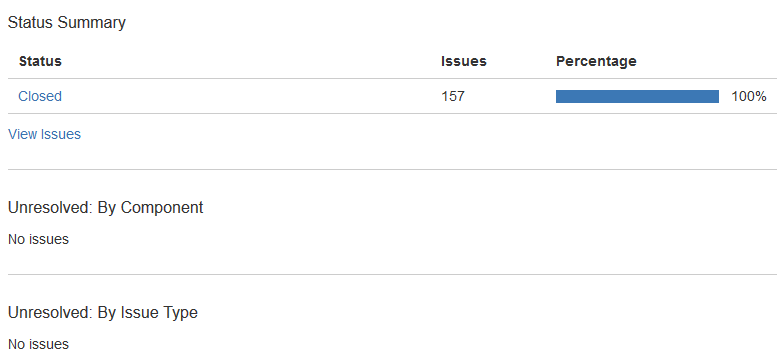
\includegraphics[scale = 0.5]{jira}
\end{center}

We took special care of the quality of the software that we built. To this end, we used Test Driven Design (TDD) and used SonarQube quality gate as a build step. We protected master branch and set up a workflow using Jenkins for continuous integration (CI). We made sure to have more than 80\% test coverage so that our application is free of bugs. 
We were very particular about addressing issues raised by the testers from other teams and managed to close all issues in time. The end product is a beautiful piece of software which we are proud to present.\par

\pagebreak
\section{The Development Process}
The project was divided into three phases, Phase A, B and C. Here is a brief description for each phase. 

\par Firstly, Phase A involved understanding the problem, gathering requirements and coming up with mock-ups and use-cases. We set up a meeting with our instructor to get to know the problem and what he was looking for. We ran by our suggestions and in the end we had a solid understanding of how to move ahead. We also researched about existing systems and brainstormed ideas to implement in the next phases. 

\par Secondly, Phase B was all about the system design. With the help of the use cases and mock-ups created in Phase A, we developed Sequence and Class Diagrams. Then, we translated them to interfaces which we would implement in the next interface. 

\par Finally, Phase C involved testing, implementing, and documenting the system. We had three sprints, lasting two weeks each, to come up with a system. 

\par Here's a brief overview of the process involved in each sprint:
\begin{enumerate}
  \item At the beginning of each sprint, we added stories and/or bugs to our backlog and estimated the stories we would be taking in the sprint. We then added them to our sprint board. 
  \item Next, we built branches corresponding to the stories on the sprint board, and started working on them locally. We moved the stories we were working on to the 'In Progress' swimlane.
  \item Once we thought that our work on the story is complete, we created a pull request on Github, asking others to test the changes. Continuous Integration via Jenkins made it possible to be sure that the master branch does not break and that all tests pass on a remote machine. 
  \item Once the PR was approved, we merged the changes from our branch to master. We then marked the story as closed on Jira. 
  \item At the end of the sprint, we had a sprint review with a TA to go over our progress in the sprint. It helped us get important feedback to do better next time.  
\end{enumerate}
\par Though we preferred face-to-face communication, we also used Slack, Teammates, and WhatsApp for communicating and co-ordinating. 

\pagebreak
\section{Project Retrospective}
We learned a lot on the way. There are a lot of things we got right and a few setbacks which are opportunities to improve. The course has made us confident enough to start working in the real world.  \par Here are some things we liked:
\begin{enumerate}
  \item We were presented with a challenging problem to solve. It forced us to think about applying Design Patterns, and writing beautiful code. 
  \item We enjoyed the DevOps role we played in the project. We not only got to code, but we also got to build the pipeline and integrate tools that helped us in the development. 
  \item Code reviews in class were helpful to both the presenter and the audience. As presenters we got valuable feedback from different perspectives, and as an audience we got to see mutual bugs which we could later identify and fix. 
\end{enumerate}
\par Here are some things which can be improved for the subsequent semesters: 
\begin{enumerate}
  \item It would be great if individual feedback is provided, in a timely manner. 
  \item It would also be helpful for teams to work on different projects. It would have more impact on their resumes.
  \item Starting the project a little earlier in the course, with a few more sprints would help the students build better software.
\end{enumerate}

\par Overall, we had a great experience with developing the project. It has helped us write better tests and implementations, and has improved our inter- and intra-team communication. 
\section{Conclusion}
We have built an application we are proud of. However, we plan to take it forward and add more features to it, and hope that instructors and TAs use our system in the semesters to come. 
\end{document}